\documentclass[a4paper,10pt]{article}
\usepackage[utf8]{inputenc}

%pour les equations
\usepackage{amsmath}
\usepackage{amssymb}
\usepackage{amsfonts}

%pour les images
\usepackage{graphicx}

% pour definir des couleurs
\usepackage{xcolor}

% pour inclure du code
\usepackage{listings}

% code color
\definecolor{ligthyellow}{RGB}{250,247,220}
\definecolor{darkblue}{RGB}{5,10,85}
\definecolor{ligthblue}{RGB}{1,147,128}
\definecolor{darkgreen}{RGB}{8,120,51}
\definecolor{darkred}{RGB}{160,0,0}

\lstset{
    language=C++,
    captionpos=b,
    extendedchars=true,
    frame=lines,
    numbers=left,
    numberstyle=\tiny,
    numbersep=5pt,
    keepspaces=true,
    breaklines=true,
    showspaces=false,
    showstringspaces=false,
    breakatwhitespace=false,
    stepnumber=1,
    showtabs=false,
    tabsize=3,
    basicstyle=\small\ttfamily,
    backgroundcolor=\color{ligthyellow},
    keywordstyle=\color{ligthblue},
    morekeywords={include, printf, uchar},
    identifierstyle=\color{darkblue},
    commentstyle=\color{darkgreen},
    stringstyle=\color{darkred},
}

%opening
\title{Mise en correspondance stéréoscopique}
\author{Elliot Vanegue}

\begin{document}

\maketitle

\section{Introduction}
Lors de ce TP, nous allons reconstituer la troisième dimension d'une image
qui a été perdu suite à la projection de celle-ci. Pour cela, nous allons 
utiliser la stéréovision afin de reconstruire la troisième dimension de certains points à
partir de deux images dont les angles de vues sont différents.

\section{Calcul de la matrice fondamentale}
La matrice fondamentale contient l'ensemble des informations de la géométrie épipolaire.
Elle est constitué de sept degrès de liberté. Cette géométrie décrit les relations entre
différentes photographies du même objet. Pour la calculer, il faut utiliser la formule suivante :
\begin{equation}
 F=(P_2O_1)^xP_2P^+_1
 \label{fondamentale}
\end{equation}
Pour calculer F, on peut voir qu'il faut utiliser un produit vectoriel afin de 
pouvoir calculer la droite passant par les points de chaque image. Pour cela,
à partir d'un vecteur p, il faut construire la matrice suivante :
\begin{equation}
 p^x=\begin{pmatrix}
  0 & -p_z & p_y\\
  p_z & 0 & -p_x\\
  -p_y & p_x & 0
 \end{pmatrix}
 \label{vectoriel}
\end{equation}

Nous allons maintenant détailler la façon de calculer la matrice fondamentale afin
d'obtenir l'équation \eqref{fondamentale}. Tout d'abord, nous devons calculer
les matrices de projection $P_1$ et $P_2$ qui sont respectivement la multiplication des matrices
intrinsèque et extrinsèque de l'image de gauche et de l'image de droite. Il faut
d'abord multiplier la matrice extrinsèque par la matrice $\begin{pmatrix} 1&0&0&0\\0&1&0&0\\0&0&1&0\end{pmatrix}$,
car la matrice extrinsèque est de la forme 4x3 alors que la matrice intrinsèque est de la forme
3x3. Ce qui nous donne le calcul suivant :
\begin{align}
 &P_1 = mLeftIntrinsic * \begin{pmatrix} 1&0&0&0\\0&1&0&0\\0&0&1&0\end{pmatrix} * mLeftExtrinsic\\
 &P_2 = mRightIntrinsic * \begin{pmatrix} 1&0&0&0\\0&1&0&0\\0&0&1&0\end{pmatrix} * mRightExtrinsic
 \label{matriceP}
\end{align}

Il ne reste plus qu'à déterminer la valeur de $O_1$ qui est un point sur l'image de gauche.
Pour calculer ces coordonnées, il faut inverser la matrice extrinsèque gauche et récupérer
les valeurs de la dernière colonne de cette matrice. Il reste alors à calculer la matrice
fondamentale avec le calcul \eqref{fondamentale}(voir \ref{Afondamentale}).

\section{Détermination d'équations de droite}
Grâce au calcul de la droite fondamentale, il est possible de déterminer les équations de droite
allant d'une image au centre de la second. Nous allons donc déterminer ces équations.
\begin{itemize}
 \item Equation de la droite épipolaire de l'image droite associée au centre de l'image de gauche :
 $F=(P_2\begin{pmatrix}u_1\\v_1\\1\end{pmatrix})^xP_2P^+_1$
 \item Equation de la droite épipolaire de l'image gauche associée au centre de l'image de droite :
 $F=(P_1\begin{pmatrix}u_2\\v_2\\1\end{pmatrix})^xP_1P^+_2$
 \item Equation de la droite épipolaire de l'image droite associée au point situé au centre du côté haut de l'image de gauche :
 $F=(P_2\begin{pmatrix}u_1\\0\\1\end{pmatrix})^xP_2P^+_1$
\end{itemize}

\section{Extraction des coins}
Nous allons maintenant mettre en évidence des pixels d'intérêt dans les deux images pour réaliser une mise
en correspondance stéréoscopique. Pour cela, nous allons utiliser la méthode de Jianbo Shi et Carlo Tomasi\cite{323794}
déjà implémenté dans la librairie OpenCV. Voici la fonction permettant de récupérer l'ensemble des coins calculés
par la fonction goodFeaturesToTrack :
\begin{lstlisting}[caption=Calcul des coins]
 Mat iviDetectCorners(const Mat& mImage,
                     int iMaxCorners) {
                   
    vector<Point2f> corners;
    goodFeaturesToTrack( mImage, corners, iMaxCorners, 0.01,
               10, Mat(), 3, false, 0.04 );

    int sizeCorners = corners.size();
    Mat mCorners = Mat(3,sizeCorners,CV_64F);

    for(int i=0; i<sizeCorners; i++) {
        mCorners.at<double>(0, i) = corners[i].x;
        mCorners.at<double>(1, i) = corners[i].y;
        mCorners.at<double>(2, i) = 1.0;
    }
    return mCorners;
}
\end{lstlisting}

Grâce à cette fonction, nous allons récupérer les coins calculés dans chaque image.
\begin{figure}[!h]
  \center
    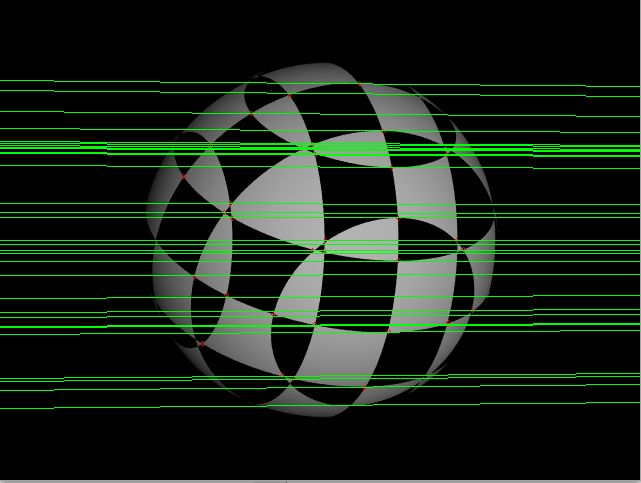
\includegraphics[width=5cm]{leftR.png}
    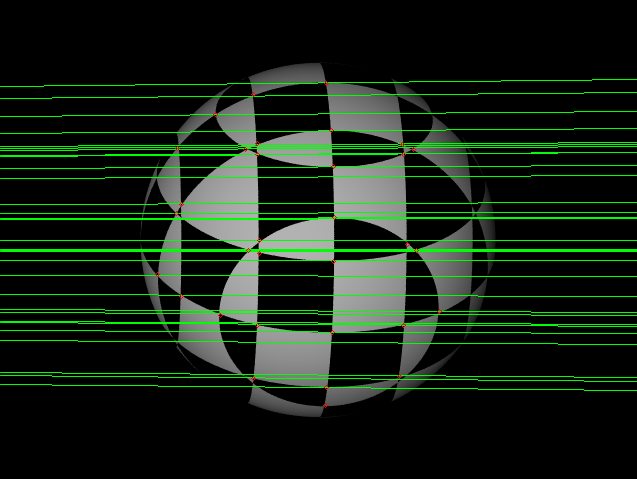
\includegraphics[width=5cm]{rightR.png}
  \caption{Mise en évidence des coins calculés avec la méthode goodFeaturesToTrack dans les images gauche et droite}
\end{figure}
%TODO voir si le fait d'avoir des points sur des lignes signifie que le point est présent dans les deux images
On peut voir, sur le résultat, des points rouge qui correspondent aux coins calculés par la méthode goodFeaturesToTrack
dans l'image, ainsi que des lignes vertes qui correspondent aux coins calculés par la méthode goodFeaturesToTrack dans la
seconde image.
 
\section{Calcul des distances}
Nous allons maintenant calculer la distance entre chaque paire de point afin de pouvoir déterminer
les meilleurs correspondances. Pour cela, nous devons calculer deux distances différentes, puis les 
additionner pour avoir le résultat final. La première distance à calculer est celle entre le point de l'image gauche et la droite épipolaire 
de l'image gauche associée au point de l'image droite. Et la seconde est celle entre le point de l'image droite et la droite épipolaire de 
l'image droite associée au point de l'image gauche. Pour cela nous allons effectuer les calcules suivants :
\begin{enumerate}
 \item $D_1 = FM_1$
 \item $D_2 = F^tM_2$
\end{enumerate}
Dans ces opération, on a $M_1$ et $M_2$ deux matrices comportant respectivement les coordonnées des points 
de l'image de gauche et de l'image de droite. En additionnant $D_1$ et $D_2$ nous obtenons l'ensemble des
distances entre chaque point.

\section{Annexes}
\subsection{Annexe A}
\label{AproduitVector}
\begin{lstlisting}[caption=Calcul produit vectoriel]
 Mat iviVectorProductMatrix(const Mat& v) {
     Mat mVectorProduct = (Mat_<double>(3,3) <<
             0.0, -v.at<double>(0,2), v.at<double>(0,1),
             v.at<double>(0,2), 0.0, -v.at<double>(0,0),
             -v.at<double>(0,1), v.at<double>(0,0), 0.0);
     return mVectorProduct;
 }
\end{lstlisting}

\subsection{Annexe B}
\label{Afondamentale}
\begin{lstlisting}[caption=Calcul matrice fondamentale]
 Mat iviFundamentalMatrix(const Mat& mLeftIntrinsic,
                         const Mat& mLeftExtrinsic,
                         const Mat& mRightIntrinsic,
                         const Mat& mRightExtrinsic) {
                         
    Mat mFundamental = Mat::eye(3, 3, CV_64F);
   
    Mat tmp = (Mat_<double>(3,4) <<
        1.0, 0.0, 0.0, 0.0,
        0.0, 1.0, 0.0, 0.0,
        0.0, 0.0, 1.0, 0.0
        );
    Mat P1 = mLeftIntrinsic * tmp * mLeftExtrinsic;
    Mat P2 = mRightIntrinsic * tmp * mRightExtrinsic;

    Mat O = mLeftExtrinsic.inv();
    Mat O1 = (Mat_<double>(4,1) <<
        O.at<double>(3),
        O.at<double>(7),
        O.at<double>(11),
        O.at<double>(15)
        );

    Mat Hpi = P2 * P1.inv(DECOMP_SVD);
    mFundamental = iviVectorProductMatrix(P2*O1) * Hpi;

    return mFundamental;
}
\end{lstlisting}

\section{Annexe C}
\label{distanceA}
\begin{lstlisting}[caption=Calcul des distances entre les points de chaque paire]
 Mat iviDistancesMatrix(const Mat& m2DLeftCorners,
                       const Mat& m2DRightCorners,
                       const Mat& mFundamental) {
 
    Mat mDistances = Mat();
    Mat d2 = mFundamental * m2DLeftCorners;
    Mat Ft = Mat();
    transpose(mFundamental, Ft);
    Mat d1 = Ft * m2DRightCorners;
    mDistances = d1 + d2;
    
    return mDistances;
}
\end{lstlisting}


\bibliographystyle{plain}
\bibliography{bibli} 

\end{document}
